\chapter{Titre de niveau 0 (chapter)}
\thispagestyle{plainNormal}


\blindtext


\section{Titre de niveau 1 (section)}
\blindtext

	\subsection{Titre de niveau 2 (subsection)}
\blindtext

\textbf{Une bien belle image se trouve \cref{fig10} \cpageref{fig10}.}

\begin{figure}[h]
\begin{center}
	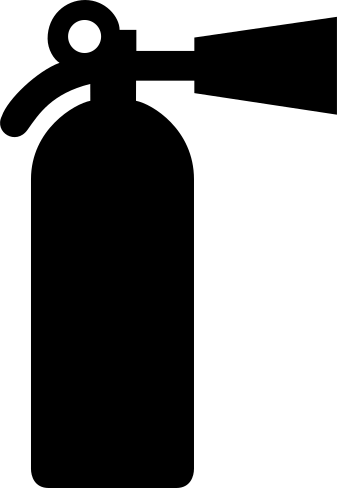
\includegraphics[width=.3\textwidth]{figures/part1/figure_10.png}
	\caption[Titre court table des matières]{Un titre beaucoup plus long et descriptif qui apparaît sous la figure.}
	\label{fig10}
\end{center}
\end{figure}

		\subsubsection{Titre de niveau 3 (subsubsection)}
\blindtext

\medskip
Liste (itemize)
\blinditemize

\medskip
Liste (enumerate)
\blindenumerate

\medskip
Liste (description)
\blinddescription

		\subsubsection{Titre de niveau 3 (subsubsection)}
\paragraph{Titre de niveau 4 (paragraph)} \blindtext

\paragraph{Titre de niveau 4 (paragraph)} \blindtext

	\subsection{Titre de niveau 2 (subsection)}
\blindtext


\section{Titre de niveau 1 (section)}
\blindtext


\clearpage
\thispagestyle{empty}